\documentclass{report}
\usepackage{tikz}
\usepackage{pdfpages}
\usetikzlibrary{matrix,calc}

\usepackage{amssymb}
\usepackage{amsmath}
\usepackage{centernot}
\usepackage{scalerel}
%\usepackage{stackengine}
\usepackage{xcolor}
\usepackage{circuitikz}
\usepackage{graphicx}
\usepackage{tkz-graph} % for drawing vector graphs
%\usepackage[margin=0.5in]{geometry}
\usepackage[top=1in,bottom=1in]{geometry}

\newcommand\showdiv[1]{\overline{\smash{\hstretch{.5}{)}\mkern-3.2mu\hstretch{.5}{)}}#1}}
\newcommand\ph[1]{\textcolor{white}{#1}}


\makeatletter
% we use \prefix@<level> only if it is defined
\renewcommand{\@seccntformat}[1]{%
  \ifcsname prefix@#1\endcsname
    \csname prefix@#1\endcsname
  \else
    \csname the#1\endcsname\quad
  \fi}
% define \prefix@section
\newcommand\prefix@section{}
\newcommand\prefix@subsection{}
\makeatother


%isolated term
%#1 - Optional. Space between node and grouping line. Default=0
%#2 - node
%#3 - filling color
\newcommand{\implicantsol}[3][0]{
    \draw[rounded corners=3pt, fill=#3, opacity=0.3] ($(#2.north west)+(135:#1)$) rectangle ($(#2.south east)+(-45:#1)$);
    }


%internal group
%#1 - Optional. Space between node and grouping line. Default=0
%#2 - top left node
%#3 - bottom right node
%#4 - filling color
\newcommand{\implicant}[4][0]{
    \draw[rounded corners=3pt, fill=#4, opacity=0.3] ($(#2.north west)+(135:#1)$) rectangle ($(#3.south east)+(-45:#1)$);
    }

%group lateral borders
%#1 - Optional. Space between node and grouping line. Default=0
%#2 - top left node
%#3 - bottom right node
%#4 - filling color
\newcommand{\implicantcostats}[4][0]{
    \draw[rounded corners=3pt, fill=#4, opacity=0.3] ($(rf.east |- #2.north)+(90:#1)$)-| ($(#2.east)+(0:#1)$) |- ($(rf.east |- #3.south)+(-90:#1)$);
    \draw[rounded corners=3pt, fill=#4, opacity=0.3] ($(cf.west |- #2.north)+(90:#1)$) -| ($(#3.west)+(180:#1)$) |- ($(cf.west |- #3.south)+(-90:#1)$);
}

%group top-bottom borders
%#1 - Optional. Space between node and grouping line. Default=0
%#2 - top left node
%#3 - bottom right node
%#4 - filling color
\newcommand{\implicantdaltbaix}[4][0]{
    \draw[rounded corners=3pt, fill=#4, opacity=0.3] ($(cf.south -| #2.west)+(180:#1)$) |- ($(#2.south)+(-90:#1)$) -| ($(cf.south -| #3.east)+(0:#1)$);
    \draw[rounded corners=3pt, fill=#4, opacity=0.3] ($(rf.north -| #2.west)+(180:#1)$) |- ($(#3.north)+(90:#1)$) -| ($(rf.north -| #3.east)+(0:#1)$);
}

%group corners
%#1 - Optional. Space between node and grouping line. Default=0
%#2 - filling color
\newcommand{\implicantcantons}[2][0]{
    \draw[rounded corners=3pt, opacity=.3] ($(rf.east |- 0.south)+(-90:#1)$) -| ($(0.east |- cf.south)+(0:#1)$);
    \draw[rounded corners=3pt, opacity=.3] ($(rf.east |- 8.north)+(90:#1)$) -| ($(8.east |- rf.north)+(0:#1)$);
    \draw[rounded corners=3pt, opacity=.3] ($(cf.west |- 2.south)+(-90:#1)$) -| ($(2.west |- cf.south)+(180:#1)$);
    \draw[rounded corners=3pt, opacity=.3] ($(cf.west |- 10.north)+(90:#1)$) -| ($(10.west |- rf.north)+(180:#1)$);
    \fill[rounded corners=3pt, fill=#2, opacity=.3] ($(rf.east |- 0.south)+(-90:#1)$) -|  ($(0.east |- cf.south)+(0:#1)$) [sharp corners] ($(rf.east |- 0.south)+(-90:#1)$) |-  ($(0.east |- cf.south)+(0:#1)$) ;
    \fill[rounded corners=3pt, fill=#2, opacity=.3] ($(rf.east |- 8.north)+(90:#1)$) -| ($(8.east |- rf.north)+(0:#1)$) [sharp corners] ($(rf.east |- 8.north)+(90:#1)$) |- ($(8.east |- rf.north)+(0:#1)$) ;
    \fill[rounded corners=3pt, fill=#2, opacity=.3] ($(cf.west |- 2.south)+(-90:#1)$) -| ($(2.west |- cf.south)+(180:#1)$) [sharp corners]($(cf.west |- 2.south)+(-90:#1)$) |- ($(2.west |- cf.south)+(180:#1)$) ;
    \fill[rounded corners=3pt, fill=#2, opacity=.3] ($(cf.west |- 10.north)+(90:#1)$) -| ($(10.west |- rf.north)+(180:#1)$) [sharp corners] ($(cf.west |- 10.north)+(90:#1)$) |- ($(10.west |- rf.north)+(180:#1)$) ;
}

%Empty Karnaugh map 4x4
\newenvironment{Karnaugh}%
{
\begin{tikzpicture}[baseline=(current bounding box.north),scale=0.8]
\draw (0,0) grid (4,4);
\draw (0,4) -- node [pos=0.7,above right,anchor=south west] {de} node [pos=0.7,below left,anchor=north east] {bc} ++(135:1);
%
\matrix (mapa) [matrix of nodes,
        column sep={0.8cm,between origins},
        row sep={0.8cm,between origins},
        every node/.style={minimum size=0.3mm},
        anchor=8.center,
        ampersand replacement=\&] at (0.5,0.5)
{
                       \& |(c00)| 00         \& |(c01)| 01         \& |(c11)| 11         \& |(c10)| 10         \& |(cf)| \phantom{00} \\
|(r00)| 00             \& |(0)|  \phantom{0} \& |(1)|  \phantom{0} \& |(3)|  \phantom{0} \& |(2)|  \phantom{0} \&                     \\
|(r01)| 01             \& |(4)|  \phantom{0} \& |(5)|  \phantom{0} \& |(7)|  \phantom{0} \& |(6)|  \phantom{0} \&                     \\
|(r11)| 11             \& |(12)| \phantom{0} \& |(13)| \phantom{0} \& |(15)| \phantom{0} \& |(14)| \phantom{0} \&                     \\
|(r10)| 10             \& |(8)|  \phantom{0} \& |(9)|  \phantom{0} \& |(11)| \phantom{0} \& |(10)| \phantom{0} \&                     \\
|(rf) | \phantom{00}   \&                    \&                    \&                    \&                    \&                     \\
};
}%
{
\end{tikzpicture}
}

% K map q2q3\Xq1
\newenvironment{KarnaughG}%
{
\begin{tikzpicture}[baseline=(current bounding box.north),scale=0.8]
\draw (0,0) grid (4,4);
\draw (0,4) -- node [pos=0.9,above right,anchor=south west] {$XQ_1$} node [pos=0.9,below left,anchor=north east] {$Q_2Q_3$} ++(135:1);
%
\matrix (mapa) [matrix of nodes,
        column sep={0.8cm,between origins},
        row sep={0.8cm,between origins},
        every node/.style={minimum size=0.3mm},
        anchor=8.center,
        ampersand replacement=\&] at (0.5,0.5)
{
                       \& |(c00)| 00         \& |(c01)| 01         \& |(c11)| 11         \& |(c10)| 10         \& |(cf)| \phantom{00} \\
|(r00)| 00             \& |(0)|  \phantom{0} \& |(1)|  \phantom{0} \& |(3)|  \phantom{0} \& |(2)|  \phantom{0} \&                     \\
|(r01)| 01             \& |(4)|  \phantom{0} \& |(5)|  \phantom{0} \& |(7)|  \phantom{0} \& |(6)|  \phantom{0} \&                     \\
|(r11)| 11             \& |(12)| \phantom{0} \& |(13)| \phantom{0} \& |(15)| \phantom{0} \& |(14)| \phantom{0} \&                     \\
|(r10)| 10             \& |(8)|  \phantom{0} \& |(9)|  \phantom{0} \& |(11)| \phantom{0} \& |(10)| \phantom{0} \&                     \\
|(rf) | \phantom{00}   \&                    \&                    \&                    \&                    \&                     \\
};
}%
{
\end{tikzpicture}
}

%Empty Karnaugh map 2x4
\newenvironment{Karnaughvuit}%
{
\begin{tikzpicture}[baseline=(current bounding box.north),scale=0.8]
\draw (0,0) grid (4,2);
\draw (0,2) -- node [pos=0.7,above right,anchor=south west] {bc} node [pos=0.7,below left,anchor=north east] {a} ++(135:1);
%
\matrix (mapa) [matrix of nodes,
        column sep={0.8cm,between origins},
        row sep={0.8cm,between origins},
        every node/.style={minimum size=0.3mm},
        anchor=4.center,
        ampersand replacement=\&] at (0.5,0.5)
{
                      \& |(c00)| 00         \& |(c01)| 01         \& |(c11)| 11         \& |(c10)| 10         \& |(cf)| \phantom{00} \\
|(r00)| 0             \& |(0)|  \phantom{0} \& |(1)|  \phantom{0} \& |(3)|  \phantom{0} \& |(2)|  \phantom{0} \&                     \\
|(r01)| 1             \& |(4)|  \phantom{0} \& |(5)|  \phantom{0} \& |(7)|  \phantom{0} \& |(6)|  \phantom{0} \&                     \\
|(rf) | \phantom{00}  \&                    \&                    \&                    \&                    \&                     \\
};
}%
{
\end{tikzpicture}
}

%Empty Karnaugh map 2x2
\newenvironment{Karnaughquatre}%
{
\begin{tikzpicture}[baseline=(current bounding box.north),scale=0.8]
\draw (0,0) grid (2,2);
\draw (0,2) -- node [pos=0.7,above right,anchor=south west] {b} node [pos=0.7,below left,anchor=north east] {a} ++(135:1);
%
\matrix (mapa) [matrix of nodes,
        column sep={0.8cm,between origins},
        row sep={0.8cm,between origins},
        every node/.style={minimum size=0.3mm},
        anchor=2.center,
        ampersand replacement=\&] at (0.5,0.5)
{
          \& |(c00)| 0          \& |(c01)| 1  \\
|(r00)| 0 \& |(0)|  \phantom{0} \& |(1)|  \phantom{0} \\
|(r01)| 1 \& |(2)|  \phantom{0} \& |(3)|  \phantom{0} \\
};
}%
{
\end{tikzpicture}
}

%Defines 8 or 16 values (0,1,X)
\newcommand{\contingut}[1]{%
\foreach \x [count=\xi from 0]  in {#1}
     \path (\xi) node {\x};
}

%Places 1 in listed positions
\newcommand{\minterms}[1]{%
    \foreach \x in {#1}
        \path (\x) node {1};
}

%Places 0 in listed positions
\newcommand{\maxterms}[1]{%
    \foreach \x in {#1}
        \path (\x) node {0};
}

%Places X in listed positions
\newcommand{\indeterminats}[1]{%
    \foreach \x in {#1}
        \path (\x) node {X};
}

\begin{document}
\includepdf{lab5_coversheet}
\section{Problem Statement}
Design a sequential circuit which adds two to a binary number in the
range 0000 through 1001. The input and output should be serial with the
least significant bit first. Find a state table with a minimum number of
states. Design the circuit using NAND gates, NOR gates, and three D
flip-flops. Any solution which is minimal for your state assignment and
uses 10 or fewer gates and inverters is acceptable.

\section {Preparatory Questions}
a. 
\includegraphics[width=400px]{time}
\\\\
b. 0 to 1, rising edge
\\\\
c. Yes, for that moment. On the rising edge, the value gets updated to the
latest version. The output may be incomplete, but it will be correct for the
values when the rising edge is triggered.
\\\\
d. No.
\\\\
e. Before. The future states of the machine may be determined by this.
\\\\
f. Before. The future states of the machine may be determined by this.
\\\\
g. Reading the output before the clock is triggered is a flawed approach. A is correct.


\section{State Table Derivations}
We start with a table of the desired states:
\\\\
\begin{tabular}{a b c d | e f g h}
\multicolumn{4}{e|}{$X$} & \multicolumn{4}{e}{$Z$} &
\hline
$t_3$ & $t_2$ & $t_1$ & $t_0$ & $t_3$ & $t_2$ & $t_1$ & $t_0$ &
\hline
0 & 0 & 0 & 0 & 0 & 0 & 1 & 0 \\
0 & 0 & 0 & 1 & 0 & 0 & 1 & 1 \\
0 & 0 & 1 & 0 & 0 & 1 & 0 & 0 \\
0 & 0 & 1 & 1 & 0 & 1 & 0 & 1 \\
0 & 1 & 0 & 0 & 0 & 1 & 1 & 0 \\
0 & 1 & 0 & 1 & 0 & 1 & 1 & 1 \\
0 & 1 & 1 & 0 & 1 & 0 & 0 & 0 \\
0 & 1 & 1 & 1 & 1 & 0 & 0 & 1 \\
1 & 0 & 0 & 0 & 1 & 0 & 1 & 0 \\
1 & 0 & 0 & 1 & 1 & 0 & 1 & 1 \\
\end{tabular} \\
\newpage
\noindent We create a truth table for the state transitions:
\\\\
\begin{tabular}{a | b | c | d e | f g}
Time & Aggregate Input & $Q$ & \multicolumn{2}{|e|}{$Q^+$} & \multicolumn{2}{e}{$Z$} &
     & (little endian) & & $X=0$ & $X=1$               & $X=0$ & $X=1$           &
\hline
$t_0$ & reset & A & B & C & 0 & 1  \\
\hline
$t_1$ & 0 & B & D & F & 1 & 0  \\
      & 1 & C & E & G & 1 & 0  \\
\hline
$t_2$ & 00 & D & H & L & 0 & 1  \\
      & 01 & E & I & M & 0 & 1  \\
      & 10 & F & J & N & 1 & 0  \\
      & 11 & G & K & P & 1 & 0  \\
\hline
$t_3$ & 000 & H & A & A & 0 & 1  \\
      & 001 & I & A & A & 0 & 1  \\
      & 010 & J & A & - & 0 & -  \\
      & 011 & K & A & - & 0 & -  \\
      & 100 & L & A & - & 0 & -  \\
      & 101 & M & A & - & 0 & -  \\
      & 110 & N & A & - & 1 & -  \\
      & 111 & P & A & - & 1 & -  \\
\end{tabular} \\
\\\\
We now have the table for state relationships. Simplfication results in:
\\\\
\begin{tabular}{a | b c | d e}
$Q$ & \multicolumn{2}{|e|}{$Q^+$} & \multicolumn{2}{e}{$Z$} &
    & $X=0$ & $X=1$               & $X=0$ & $X=1$           &
\hline
A & B & B & 0  & 1  \\
B & D & F & 1  & 0  \\
D & H & H & 0  & 1  \\
F & H & N & 1  & 0  \\
H & A & A & 0  & 1  \\
N & A & - & 1  & -  \\
\end{tabular} \\
\\\\
This table can get Boolean expressions for logic.


\section{State Machine Design}
Initially, we will start the circuit in a reset state designated $A$
($A000$ in the graph). The first input bit will be echoed back out and
$A$ will always transition to $B$ (depicted as $B001$).

When in state $B$, the next bit given will be flipped on output. If a 1 is
received, then $B$ transitions to $F$ (depicted $F011$), else $D$ (depicted
$D010$).

After this, $D$ will always transition to $H$ (depicted $H011$) since $D$
represents the state where 0 is in the 2's place. The input is simply echoed
in this state.

If the current state is $F$, then there may be a carry to deal with. If the
next input bit is 0, then $F$ transitions to $H$ while echoing the input
value. However, if the input bit while in state $F$ is 1, then $F$
transitions to $N$ (depicted below as $N101$), outputting 0. $N$ represents
the state where the three least significant bits were $X11$ (little endian)
and a carry bit is needed in the most significant output digit.

Finally, $H$ and $N$ always go back to the reset state $A$. $H$ has no carry,
so input is echoed to output. $N$ has a carry, so the bit is flipped. Note
that $N$ never receives a 1, by constraint of our problem. However, it would
be reasonable to let it still transition to $A$ while outputting a 0 if 1 was
received (not implemented here).


\section{State Graph}
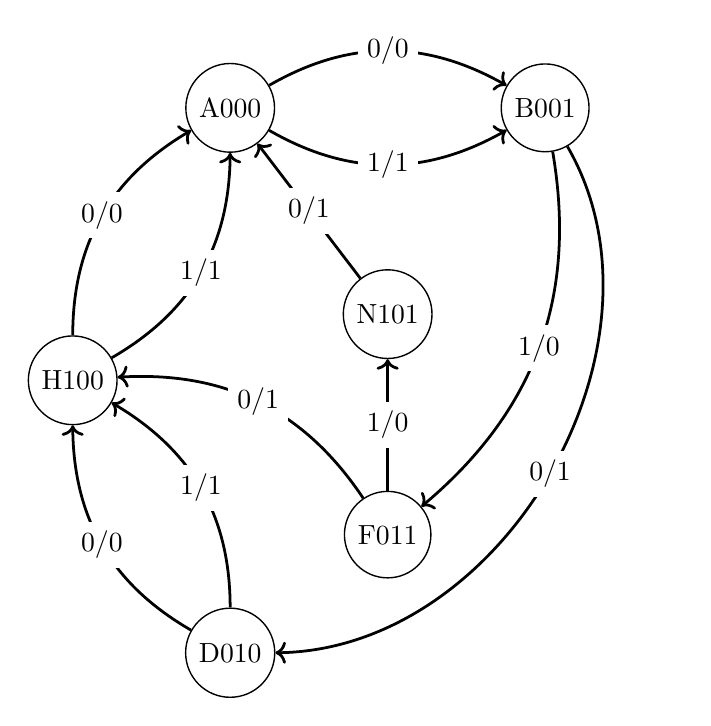
\begin{tikzpicture}
 \SetUpEdge[lw         = 1.0pt,
            color      = black,
            labelcolor = white]
  \GraphInit[vstyle=Normal] 
  \SetGraphUnit{3}
  \tikzset{VertexStyle/.append  style={fill}}
  \Vertex[x=2,y=6.92]{A000}
  \Vertex[x=6,y=6.92]{B001}
  \Vertex[x=0,y=3.46]{H100}
  \Vertex[x=4,y=4.3]{N101}
  \Vertex[x=2,y=0]{D010}
  \Vertex[x=4,y=1.5]{F011}

  % A
  \tikzset{EdgeStyle/.style={->,relative=true,in=150,out=30}}
    \Edge[label=$0/0$](A000)(B001)
  \tikzset{EdgeStyle/.style={->,relative=true,in=210,out=-30}}
    \Edge[label=$1/1$](A000)(B001)

  % B
  \tikzset{EdgeStyle/.style={->,bend left=60}}
    \Edge[label=$0/1$](B001)(D010)
  \tikzset{EdgeStyle/.style={->,bend left=30}}
    \Edge[label=$1/0$](B001)(F011)

  % D
  \tikzset{EdgeStyle/.style={->,relative=true,in=150,out=30}}
    \Edge[label=$0/0$](D010)(H100)
  \tikzset{EdgeStyle/.style={->,relative=true,in=210,out=-30}}
    \Edge[label=$1/1$](D010)(H100)

  % F
  \tikzset{EdgeStyle/.style={->,relative=true,in=210,out=-30}}
    \Edge[label=$0/1$](F011)(H100)
  \tikzset{EdgeStyle/.style={->}}
    \Edge[label=$1/0$](F011)(N101)

  % H
  \tikzset{EdgeStyle/.style={->,relative=true,in=150,out=30}}
    \Edge[label=$0/0$](H100)(A000)
  \tikzset{EdgeStyle/.style={->,relative=true,in=210,out=-30}}
    \Edge[label=$1/1$](H100)(A000)

  % N
  \tikzset{EdgeStyle/.style={->}}%,relative=true,in=150,out=30}}
    \Edge[label=$0/1$](N101)(A000)
  %\tikzset{EdgeStyle/.style={->}}%,relative=true,in=210,out=-30}}
    %\Edge[label=$1/0$](N011)(X)
\end{tikzpicture}


\section{LogicAid}
The desired data is entered into LogicAid:

\includegraphics[width=200px]{states}


\section{State Assignment}
After verification, we perform a state assignment - specifically we select the
initial reset state $A$ to be encoded as flip-flop state 000, $B$ to be 100,
$D$ to be 101, $F$ to be 111, $H$ to be 110, and $N$ to be 001. $Z$ represents
output, $X$ an input bit, $Q_n$ the $n^{th}$ bit, and $Q_n^+$ the next $n^{th}$
bit. The following is the transition table after the state assignment:
\\\\
\begin{tabular}{z | a | b c | d e}
 & $Q_1Q_2Q_3$ & \multicolumn{2}{|e|}{$Q_1^+Q_2^+Q_3^+$} & \multicolumn{2}{e}{Z} &
 &  & $X=0$ & $X=1$ & $X=0$ & $X=1$ &
\hline
A & 000 & 001 & 001 & 0  & 1  \\
B & 001 & 010 & 011 & 1  & 0  \\
D & 010 & 100 & 100 & 0  & 1  \\
F & 011 & 100 & 101 & 1  & 0  \\
H & 100 & 000 & 000 & 0  & 1  \\
N & 101 & 000 & -   & 1  & -  \\
\end{tabular} \\
\\\\
The state assignment in LogicAid is shown below:

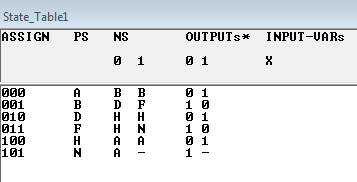
\includegraphics[width=200px]{astates}

\section{Equations}
From the transition table, we plot the next-state maps for the flip-flops and the map for the output function Z and derive the equations for $Q_1^+$, $Q_2^+$, $Q_3^+$, and Z:
\\\\
\indent $Q_1^+ = Q_2$ \\
\begin{KarnaughG}
    \contingut{0,0,0,0,0,0,0,X,1,X,1,X,1,X,1,X}
    \implicant{12}{10}{green}
\end{KarnaughG}

\\\\
$Q_2^+ = Q_1'Q_2'Q_3
= (Q_1 + Q_2 + Q_3')'
= \downarrow (Q_1, Q_2, Q_3') $ \\
\begin{KarnaughG}
    \contingut{0,0,0,0,1,0,1,X,0,X,0,X,0,X,0,X}
    \implicantcostats{4}{6}{purple}
\end{KarnaughG}

\newpage
\\
$Q_3^+
= Q_1'Q_2'Q_3' + XQ_3
= ((Q_1'Q_2'Q_3')'(XQ_3)')'
= \uparrow (\uparrow (Q_1', Q_2', Q_3'), \uparrow (X, Q_3))$ \\
\begin{KarnaughG}
    \contingut{1,0,1,0,0,0,1,X,0,X,0,X,0,X,1,X}
    \implicantcostats{0}{2}{purple}
    \implicant{7}{14}{green}
\end{KarnaughG}

\\\\
$Z = X'Q_3 + XQ_3'
= ((X'Q_3)'(XQ_3')')'
= \uparrow (\uparrow (X', Q_3), \uparrow (X, Q_3'))$ \\
\begin{KarnaughG}
    \contingut{0,0,1,1,1,1,0,X,0,X,1,X,1,X,0,X}
    \implicant{4}{13}{green}
    \implicantdaltbaix{3}{10}{orange}
\end{KarnaughG}

\newpage
\section{Circuit}
Below is a schematic of the circuit in SimUaid:

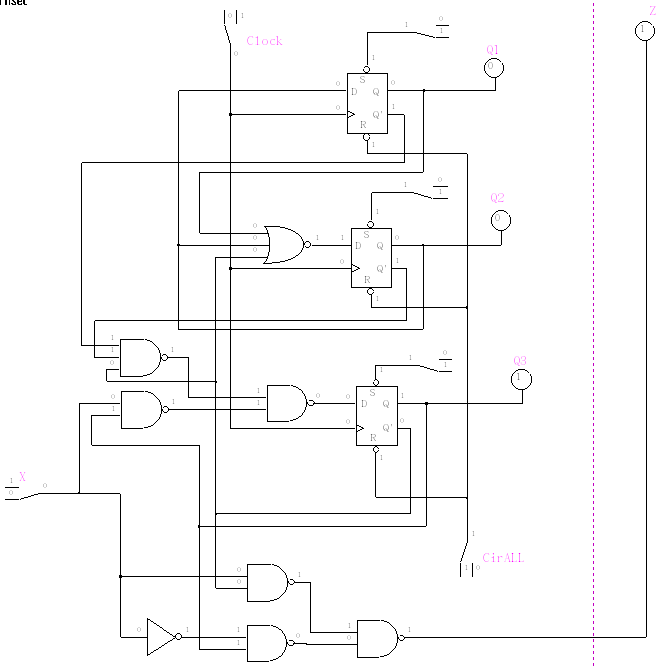
\includegraphics[width=400px]{ckt}



\end{document}
